% File: template.tex
% InputFile: packages.tex
\documentclass[11pt,a4paper]{article}
% Packages per la formattazione
%package per le sezioni a quattro indici
\usepackage{titlesec} 
\usepackage[left=3.5cm,right=3.5cm,top=3.1cm,bottom=2.6cm]{geometry}
\usepackage[italian]{babel}
\usepackage[utf8]{inputenc}
\usepackage{lastpage}
\usepackage[T1]{fontenc}
\usepackage{geometry}
%package per la gestione delle immagini
\usepackage{graphicx}
%pakage per ridefinire font caption
\usepackage[font=small,labelfont=bf]{caption} 
\geometry{a4paper}
%package di style per  l/c/rhead l/rfoot
\usepackage{fancyhdr} 

%package per i punti nella tableofcontents
\usepackage{tocloft} 
\usepackage{longtable}
\pagestyle{fancy}

% package per i colori
\usepackage{color} 
\usepackage[table]{xcolor} 
\definecolor{acqua}{rgb}{0.0, 1.0, 1.0}

\usepackage{hyperref}
\hypersetup {
	colorlinks=true,
	linkcolor=black
}		 

%package meno complesso per la gestione delle tabelle
\usepackage{tabularx}
\usepackage{pdfpages}
%package per il simbolo dell'euro
\usepackage{eurosym}
%package per unire 2 righe
\usepackage{multirow}
%package per mettere il foglio in orizzontale 
 \usepackage{pdflscape}
\usepackage{titlesec}
\usepackage{epstopdf}
\usepackage{makecell}
	
% Indentazione prima linea dei paragrafi
\usepackage{indentfirst}

%indice con i puntini
\usepackage{tocloft}
\renewcommand\cftsecleader{\cftdotfill{\cftdotsep}}
% InputFile. commands.tex

%%INSERT HERE THE NAME OF THE EDITORS
\newcommand{\fiamma}{Fiammetta Cannavò}
\newcommand{\ludo}{Lorenzo Dei Negri}
\newcommand{\perin}{Federico Perin}
\newcommand{\toffo}{Massimo Toffoletto}

% BASE COMMANDS 
\newcommand{\data}{\today}

% package per il background
\usepackage[pages=some]{background}

\newcommand{\cover}{
	\begin{titlepage}
		\begin{center}
		
			\BgThispage
			\thispagestyle{empty}
			
			\begin{figure}
				\begin{center}
					
\includegraphics[width=11cm]{img/Logo} 
				\end{center}
			\end{figure}	
			
			\vspace{3cm}
			
			\begin{Huge}
				\textbf{Museo \textit{TecArt} \\ Relazione di progetto} \\
			\end{Huge}
			
			\vspace{9pt}  
			
			\begin{large}
				\textbf{Progetto universitario di Tecnologie Web\\}
				\textbf{Anno accademico 2019/2020}\\
				\vspace{3pt}
			\end{large}	  
			
			\vspace{20pt}
			
      	\begin{large}
        	\textbf{Riferimenti progetto\\}
        	\textbf{Indirizzo sito web:} %\emph{http://tecweb1920.studenti.math.unipd.it/mdallali}
       		\\
        	\textbf{Repository GitHub:} %\emph{https://github.com/marcoDallas/TECWEB1920}\\
      \end{large} 

      \vspace{10pt} 
      
     \begin{center}
     	\textbf{Componenti del gruppo}\\ \bigskip
		\begin{tabular}{ l | c }
				Studente 	& Matricola \\ \hline 
		 		\fiamma 		& 1167703 \\ 
		 		\ludo 			& 1161729 \\ 
		 		\perin 			& 1170747\\ 
				\toffo			& 1161727 \\
			\end{tabular}
			\vspace{0.5cm}
		\end{center}

		\vspace*{\fill}
			
		\begin{center}
			\textbf{Referente\\}
%			Dalla Libera Marco - marco.dallalibera.2@studenti.unipd.it\\
%			\textbf{Utente\\}
%			\textit{Amministratore:} admin - admin\\
		\end{center}
			
		\end{center}
	\end{titlepage}
\pagebreak
}	%FINE NEW COMMAND COPERTINA


\pagestyle{fancy}
\fancyhf{}
\setlength\headheight{50pt}
\rhead{ Relazione di Progetto }
\lhead{
\includegraphics[scale=0.07]{img/Logo}}
\cfoot{\thepage \ di \pageref{LastPage}}

% Linea nel footer 
\renewcommand{\footrulewidth}{0.4pt}

% 3 e 4 livello di profondita' per section e ToC
\setcounter{secnumdepth}{4}
\setcounter{tocdepth}{4}
\titleformat{\paragraph}
{\normalfont\normalsize\bfseries}{\theparagraph}{1em}{}
\titlespacing*{\paragraph}
{0pt}{3.25ex plus 1ex minus .2ex}{1.5ex plus .2ex}

%% Indentazione prima linea dei paragrafi
%\usepackage{indentfirst}
%
%%indice con i puntini
%\usepackage{tocloft}
%\renewcommand\cftsecleader{\cftdotfill{\cftdotsep}}

% background setup
\backgroundsetup {
	scale=1,
	color=white,
	opacity=0,
	angle=0
}	

\begin{document}
	% <<<<< MODIFICARE
		
	%\input{firstpage}
	\cover
 	
	\pagebreak
	\tableofcontents % indice
	\thispagestyle{fancy}
	\pagebreak
	
	 %Contenuto del documento % <<<<< MODIFICARE
	
	\section{Abstract}
\label{abstract}
\textit{TecArt} è un museo d'arti figurative specializzato in dipinti e sculture di autori italiani ed europei dal XV secolo in poi. Il sito offre al visitatore la possibilità di consultare agevolmente l'elenco di alcune tra le opere più significative esposte nella sede del museo: in pochi click l'utente può consultare la scheda completa di pezzi prestigiosissimi. È possibile anche restare aggiornati sugli eventi artistici che saranno ospitati dal museo. Le opere sono classificate in \textit{dipinti} e \textit{sculture}, gli eventi in \textit{mostre} e \textit{conferenze}.

Oltre ad opere ed eventi, ad un breve estratto della storia del museo e alle indicazioni per contattare o raggiungere la sede, il sito raccoglie le recensioni lasciate dai visitatori, per garantire la massima trasparenza verso gli utenti e mostrare i feedback ricevuti sul servizio offerto.

Infine, in qualunque momento il visitatore può cercare il contenuto desiderato tramite la barra di ricerca messa a disposizione da tutte le pagine del sito.

Qualora si verificasse un errore durante la navigazione, l'utente viene mandato su una pagina di recupero, che gli permette di tornare alla \textit{Home page}, oltre che di navigare attraverso il menu o usufruire della funzionalità di ricerca.

L'utente affezionato, o semplicemente soddisfatto dell'esperienza nel museo, ha la possibilità di registrarsi e crare un account nel sito tramite la compilazione di un semplice form: in questo modo potrà rilasciare delle recensioni, modificarle o rimuoverle.

L'utente amministratore potrà aggiungere, modificare o rimuovere le informazioni relative agli eventi e alle opere, cancellare gli account degli utenti indesiderati e rimuovere le recensioni ritenute inappropriate.

Ogni aspetto del sito è stato pensato per garantire una navigazione semplice e gradevole alla più vasta utenza possibile, prestando particolare attenzione alla scelta della struttura, del \textit{layout}, dei colori e di tutti gli aspetti legati all'accessibilità.
	\pagebreak
	\section{Analisi}
\label{analisi}

\subsection{Categorie di utenti}
\label{analisi-categorie-utenti}
Il museo si rivolge ad un'utenza molto ampia: le opere esposte possono attirare scolaresche, docenti, amatori, specialisti del settore, famiglie, anziani.

Gli utenti specialisti o appassionati d'arte sono interessati al lato tecnico e critico delle opere: le schede descrittive dovranno quindi essere ben curate e l'esposizione delle informazioni chiara e precisa. Famiglie e scolaresche puntano ad un'esperienza meno appronfondita ma più ampia e didattica: la collezione di opere presentate deve quindi essere ampia e variegata, e gli eventi organizzati devono prevedere mostre e cicli di conferenze sul più ampio spettro di correnti e tematiche artistiche possibile.

In generale, il sito deve essere pronto a corrispondere alle esigenze di un'utenza varia e ampia: l'interfaccia deve essere intutiva e leggibile, la terminologia non troppo specialistica, la grafica adatta ad un pubblico di tutte le età, nè troppo seria nè eccessivamente giocosa.

\subsubsection{Attori principali}
\label{analisi-casi-uso-attori-principali}
Sono state individuate tre categorie principali di attori: \textit{utente generico}, \textit{utente autenticato}, \textit{utente ammininstratore}.

L'\textit{utente generico} è un visitatore anonimo del sito, che non ha effettuato né registrazione né login; egli ha la possibilità di interagire col sito mediante il form di registrazione, la barra di ricerca e i filtri di visualizzazione di opere ed eventi. L'utente generico può prendere visione di tutti i contenuti senza però poterli modificare, eliminare e senza poterne aggiungere di nuovi.

L'\textit{utente autenticato} eredita tutte le funzionalità dell'utente generico. In aggiunta, avendo un account personale nel database, può accedere alla propria area utente, gestire i propri dati personali, lasciare recensioni, modificarle ed eliminarle.

L'\textit{utente amministratore} eredita anch'esso le funzionalità di quello generico, cui si aggiungono quelle legate al possesso di un account (visualizzazione dei dati personali e loro modifica, come per l'\textit{utente autenticato}) e  la gestione di tutti i contenuti presenti nel sito. L'amministratore può inserire, modificare e rimuovere le pagine relative ad eventi e opere, e eliminare, se necessario, recensioni o account di utenti indesiderati.


\subsection{Casi d'uso}
\label{analisi-casi-uso}

\subsubsection{Utente generico}
\label{analisi-casi-uso-attori-principali-utente-generico}
I casi d'uso che riguardano questa categoria di utenti sono:
\begin{itemize}
	\item visualizzazione \textit{Home page};
	\item interazione coi link del \textit{breadcrumb};
	\item visualizzazione della pagina \textit{Opere};
	\item interazione con la pagina \textit{Opere};
	\item visualizzazione della pagina \textit{Eventi};
	\item interazione con la pagina \textit{Eventi};
	\item visualizzazione della pagina \textit{Cosa dicono di noi};
	\item interazione con la pagina \textit{Cosa dicono di noi};
	\item visualizzazione della pagina \textit{Contatti};
	\item visualizzazione della pagina \textit{Login};
	\item esecuzione di una ricerca mediante la barra nell'\textit{header};
	\item visualizzazione risultato della ricerca nella pagina \textit{Ricerca};
	\item interazione con la pagina \textit{Ricerca};
	\item visualizzazione della pagina \textit{Opera};
	\item visualizzazione della pagina \textit{Evento};
	\item visualizzazione della pagina \textit{Recensione};
	\item visualizzazione della pagina \textit{Registrazione};
	\item creazione di un account dalla pagina \textit{Registrazione};
	\item visualizzazione della pagina di \textit{Errore}.
\end{itemize}

\subsubsection{Utente autenticato}
\label{analisi-casi-uso-attori-principali-utente-autenticato}
Oltre a tutti i casi d'uso esposti per l'utente generico, riguardano l'utente autenticato anche:
\begin{itemize}
	\item autenticazione dalla pagina \textit{Login};
	\item visualizzazione della pagina \textit{Utente};
	\item inserimento di una recensione dalla pagina \textit{Lascia una recensione};
	\item visualizzazione delle proprie recensioni dalla pagina \textit{Gestione recensioni};
	\item modifica di una recensione dalla pagina \textit{Gestione recensioni};;
	\item visualizzazione della pagina \textit{Recensione modificata};
	\item eliminazione di una recensione dalla pagina \textit{Gestione recensioni};
	\item modifica dei propri dati utente dalla pagina \textit{Modifica dati utente};
	\item visualizzazione della pagina \textit{Dati utente modificati};
	\item logout dal proprio account.
\end{itemize}

\subsubsection{Utente amministratore}
\label{analisi-casi-uso-attori-principali-utente-amministratore}
Oltre a tutti i casi d'uso esposti per l'utente generico, riguardano l'utente amministratore anche:
\begin{itemize}
	\item autenticazione dalla pagina \textit{Login};
	\item visualizzazione della pagina \textit{Utente};
	\item visualizzazione della pagina \textit{Gestione contenuti};
	\item interazione con la pagina \textit{Gestione dei contenuti};
	\item modifica dei dati di un'opera dalla pagina \textit{Modifica opera};
	\item modifica dei dati di un evento dalla pagina \textit{Modifica evento};
	\item rimozione di un evento o un'opera dal sito dalla pagina \textit{Gestione contenuti};
	\item rimozione di una recensione dal sito dalla pagina \textit{Gestione recensioni};
	\item rimozione di un utente dal sito dalla pagina \textit{Gestione utenti};
	\item logout dal proprio account.
\end{itemize}

	\pagebreak
	\section{Progettazione}
\label{progettazione}

\subsection{Database}
\label{progettazione-database}
Il database di appoggio per i contenuti del sito si articola in quattro tabelle. 

La tabella \textit{Utenti} memorizza i dati degli utenti che effettuano la registrazione sul sito; vi appartengono sia gli utenti autenticati che gli utenti amministratori, questi ultimi distinti dal attributo \textit{Admin}, posto ad 1 se l'utente è amministratore.

La tabella \textit{Opere} contiene i dati relativi alle opere presentate nel sito. Di ognuna vengono presentati i dati tecnici, la descrizione e se si tratta di un prestito o di un pezzo permanente della collezione; a questa tabella appartengono sia \textit{dipinti} che \textit{sculture}. Se fosse necessario, in futuro, prevedere altri tipi di opere artistiche, sarebbe sufficiente aggiungere elementi all'attributo "stile" e gli eventuali attributi specifici del nuvo tipo introdotto.

La tabella \textit{Eventi} contiene i dati relativi agli eventi organizzati dal museo. Di ognuno sono riportati i dati logistici e la descrizione; a questa tabella appartengono sia le \textit{conferenze}, previste anche in cicli, che le \textit{mostre}. Se in futuro venissero programmati eventi di altro tipo, per memorizzarli basterebbe aggiungerne la tipologia all'omonimo attributo della tabella, insieme adf altri evenutali attributi specifici dell'evento organizzato.

Infine, la tabella \textit{Recensione} tiene traccia delle recensioni inserite nel sito dagli utenti autenticati. Poiché è previsto che un utente possa modificare una recensione precedentemente inserita, ne viene mantenuta la data di utlima modifica.

\textit{Utenti} è in relazione con le altre tre classi: di ciascun tipo di contenuto previsto, infatti, si memorizza l'utente che ha effettuato l'inserimento. Per \textit{Opere} ed \textit{Eventi} si tratta sempre di un \textit{utente amministratore}, per le recensioni è sempre un \textit{utente autenticato}.

\begin{center}
	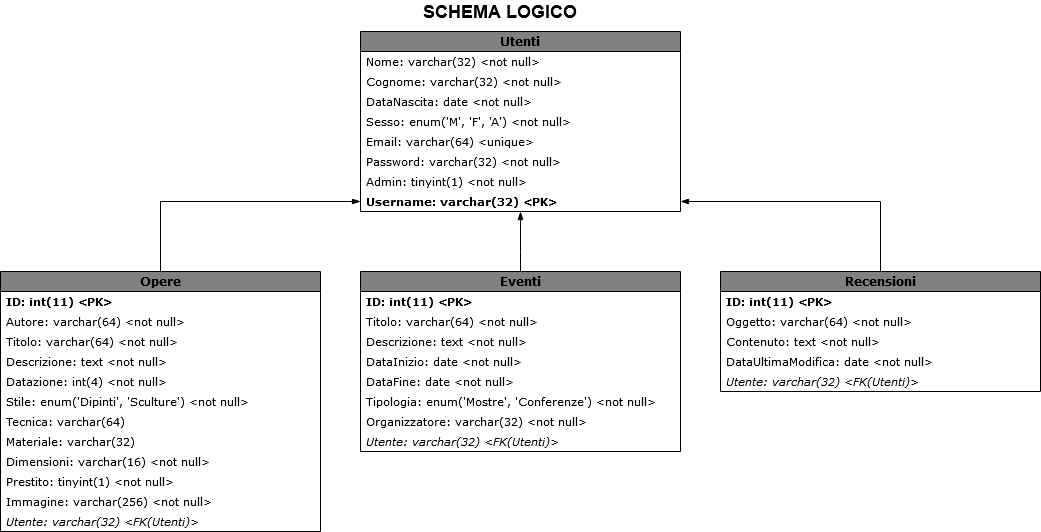
\includegraphics[width=\textwidth]{img/SchemaLogico}
	\captionof{figure}{Schema logico del database del museo \textit{TecArt}}
\end{center}

\subsection{\textit{Layout}}
\label{progettazione-layout}
Per la scelta del design delle pagine, l'obiettivo è l'adattabilità al maggior numero possibile di dispositivi, indipendentemente dalle dimensioni dello schermo o dal supporto usato dall'utente. Si è puntato poi ad avere una struttura ordinata, leggera e di immediata comprensione e memorizzazione, al fine di rendere la navigazione semplice e intuitiva.
Per soddisfare queste esigenza è stato scelto il "\textit{layout} a tre pannelli". Come da struttura standard, questo tipo di layout divide la schermata in tre settori: \textit{header} che deve contenere la rispota alla domanda "dove mi trovo?"; \textit{menu}, che deve contenere la rispota alla domanda "dove posso andare?"; \textit{content}, che deve contenere la rispota alla domanda "cosa c'è nella pagina?".
\begin{itemize}
	\item \textit{Header:} su desktop, tablet e mobile occupa la fascia superiore della finestra ed è ampio quanto tutta la schermata. Riporta il nome del sito, il menu per l'accesso all'aera personale e la barra di ricerca. Nella parte più bassa contiene il \textit{breadcrumb}, che indica il percorso fatto dal visitatore all'interno del sito per arrivare alla pagina corrente. Per permettere agilmente all'utente di tornare alla pagine visitate in precedenza, il \textit{breadcrumb} si compone dei link delle pagine corrispondenti. 
	\item \textit{Menu}: riporta i link alle pagine principali del sito, contenenti tutte le informazioni rilevanti per la più ampia categoria di utenti.
	\item \textit{Content}: presenta il contenuto effettivo della pagina.
\end{itemize}
Nella parte più bassa della finestra, simmetricamente all'\textit{header}, si trova il \textit{footer}, che riporta le immagini certificanti la validazione, alcuni dettagli didattici e gli autori del sito. \\\\

In base alle dimensioni della finestra, questi elementi vengono visualizzati in modo diverso. A seguire, un esempio di design per i formati \textit{mobile}, \textit{tablet} e \textit{desktop}.

\begin{center}
	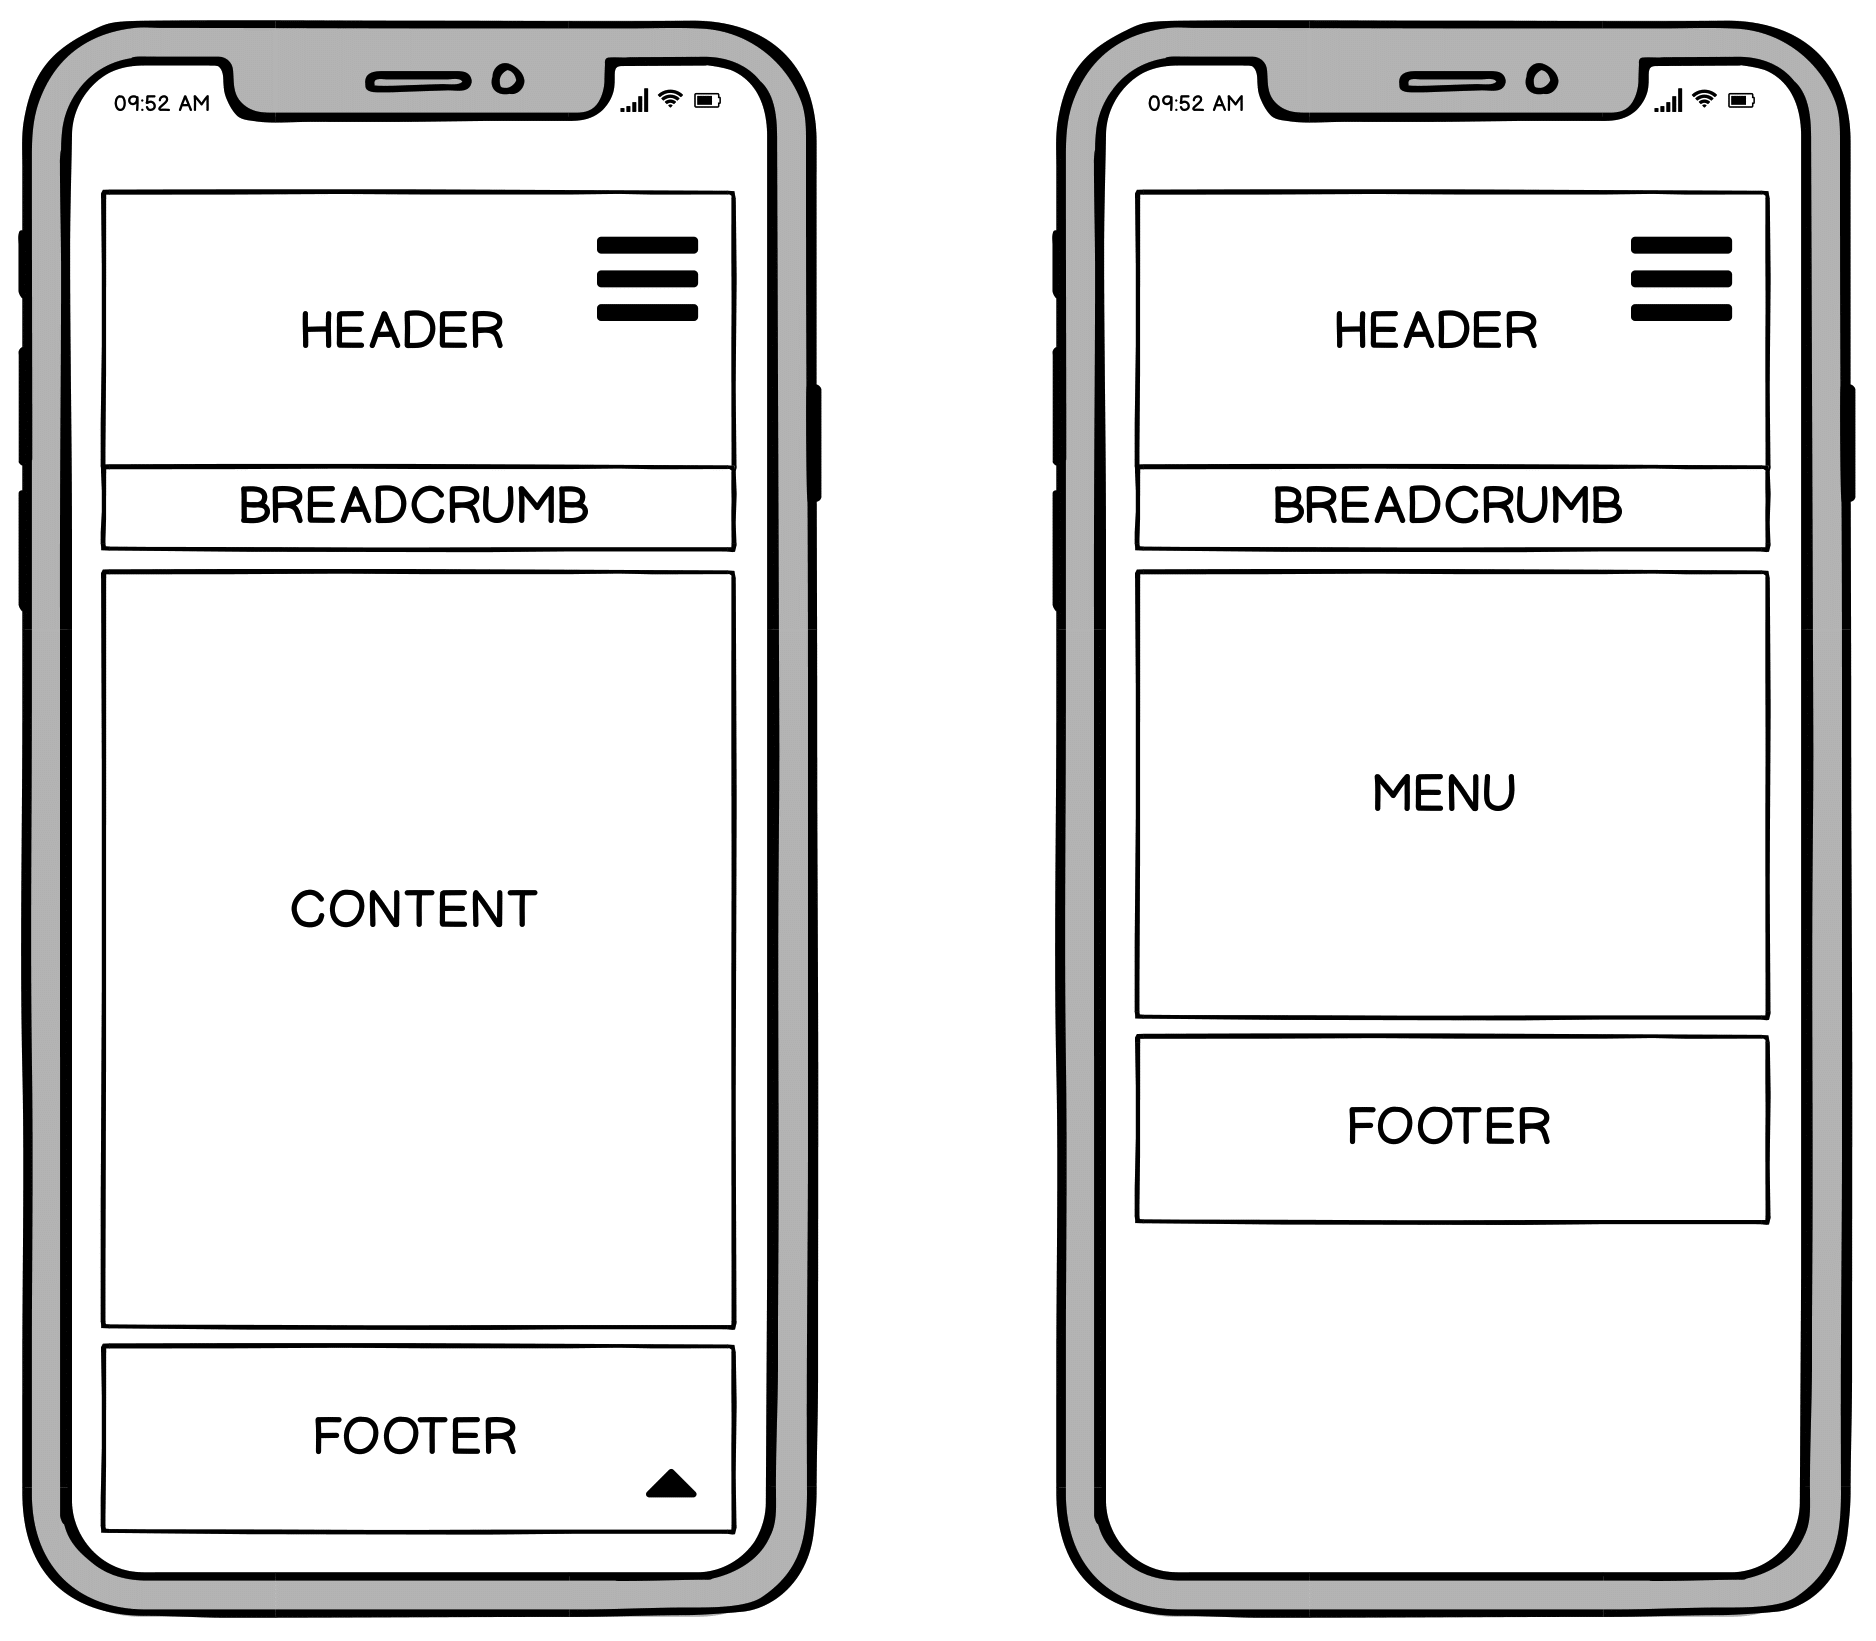
\includegraphics[scale=0.15]{img/Mobile}
	\captionof{figure}{\textit{Layout mobile} con \textit{menu} nascosto (a sinistra) e visibile (a destra)}
\end{center}

\begin{center}
	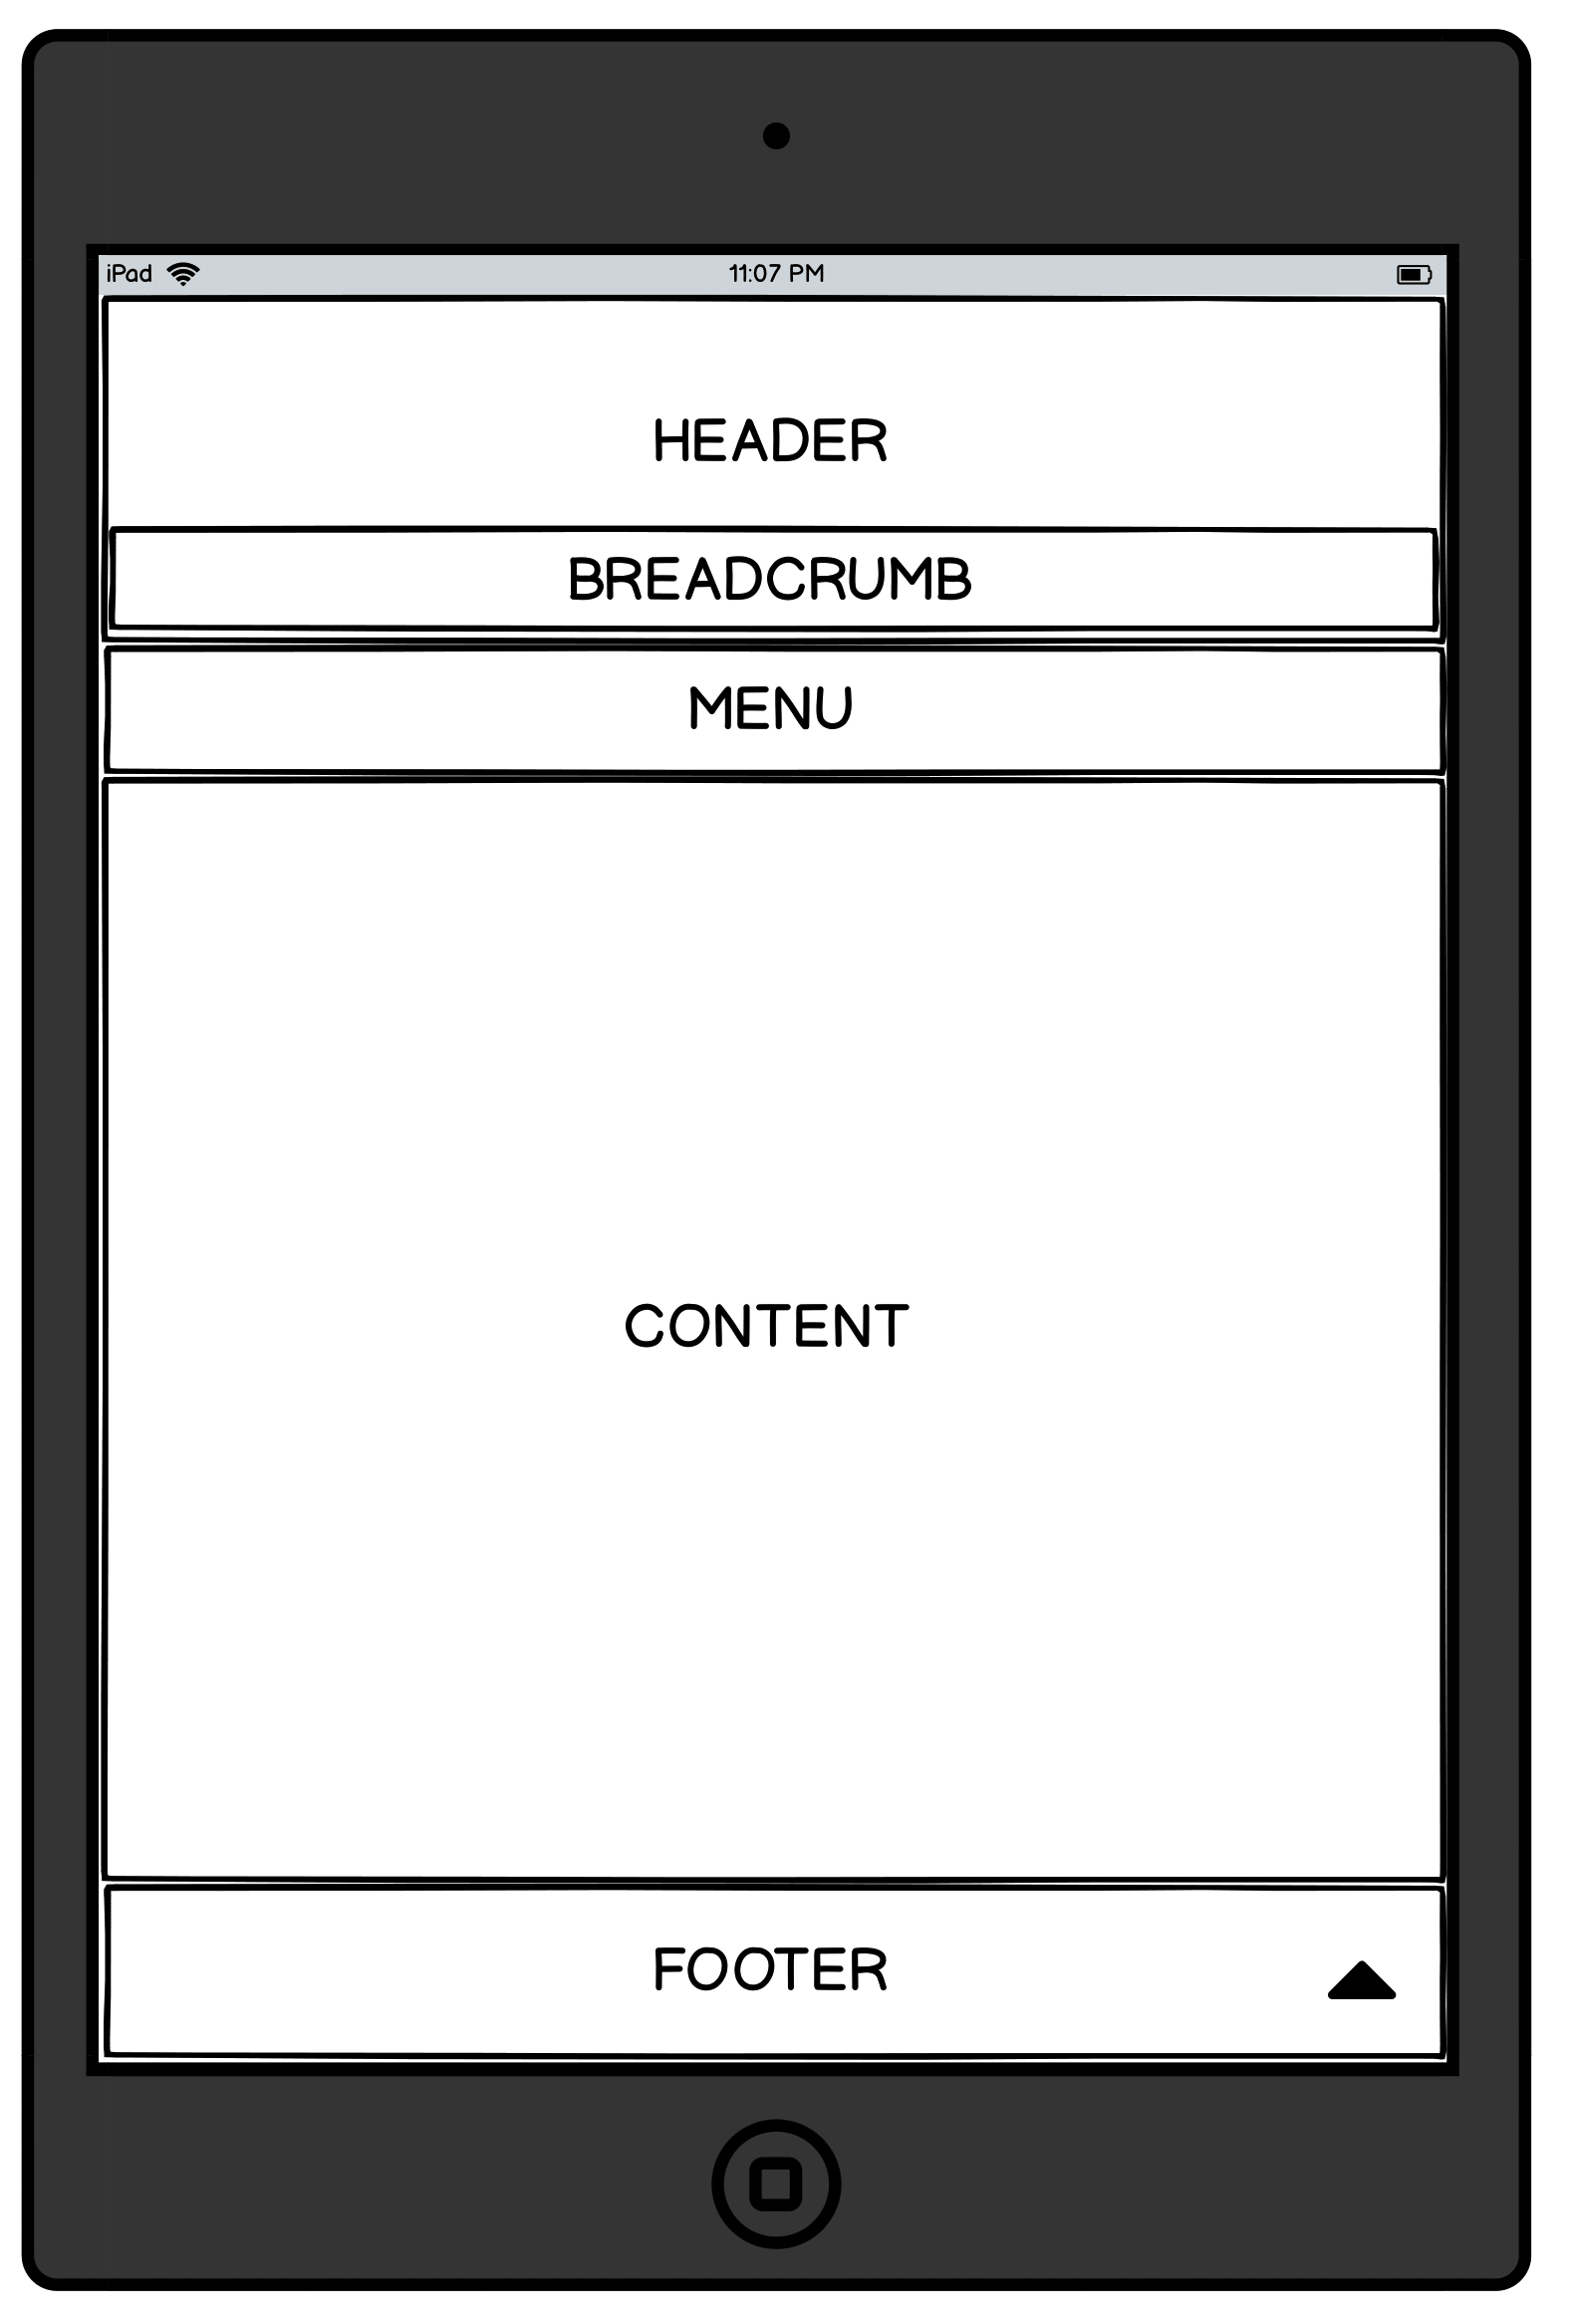
\includegraphics[scale=0.13]{img/Tablet}
	\captionof{figure}{\textit{Layout tablet}}
\end{center}

\begin{center}
	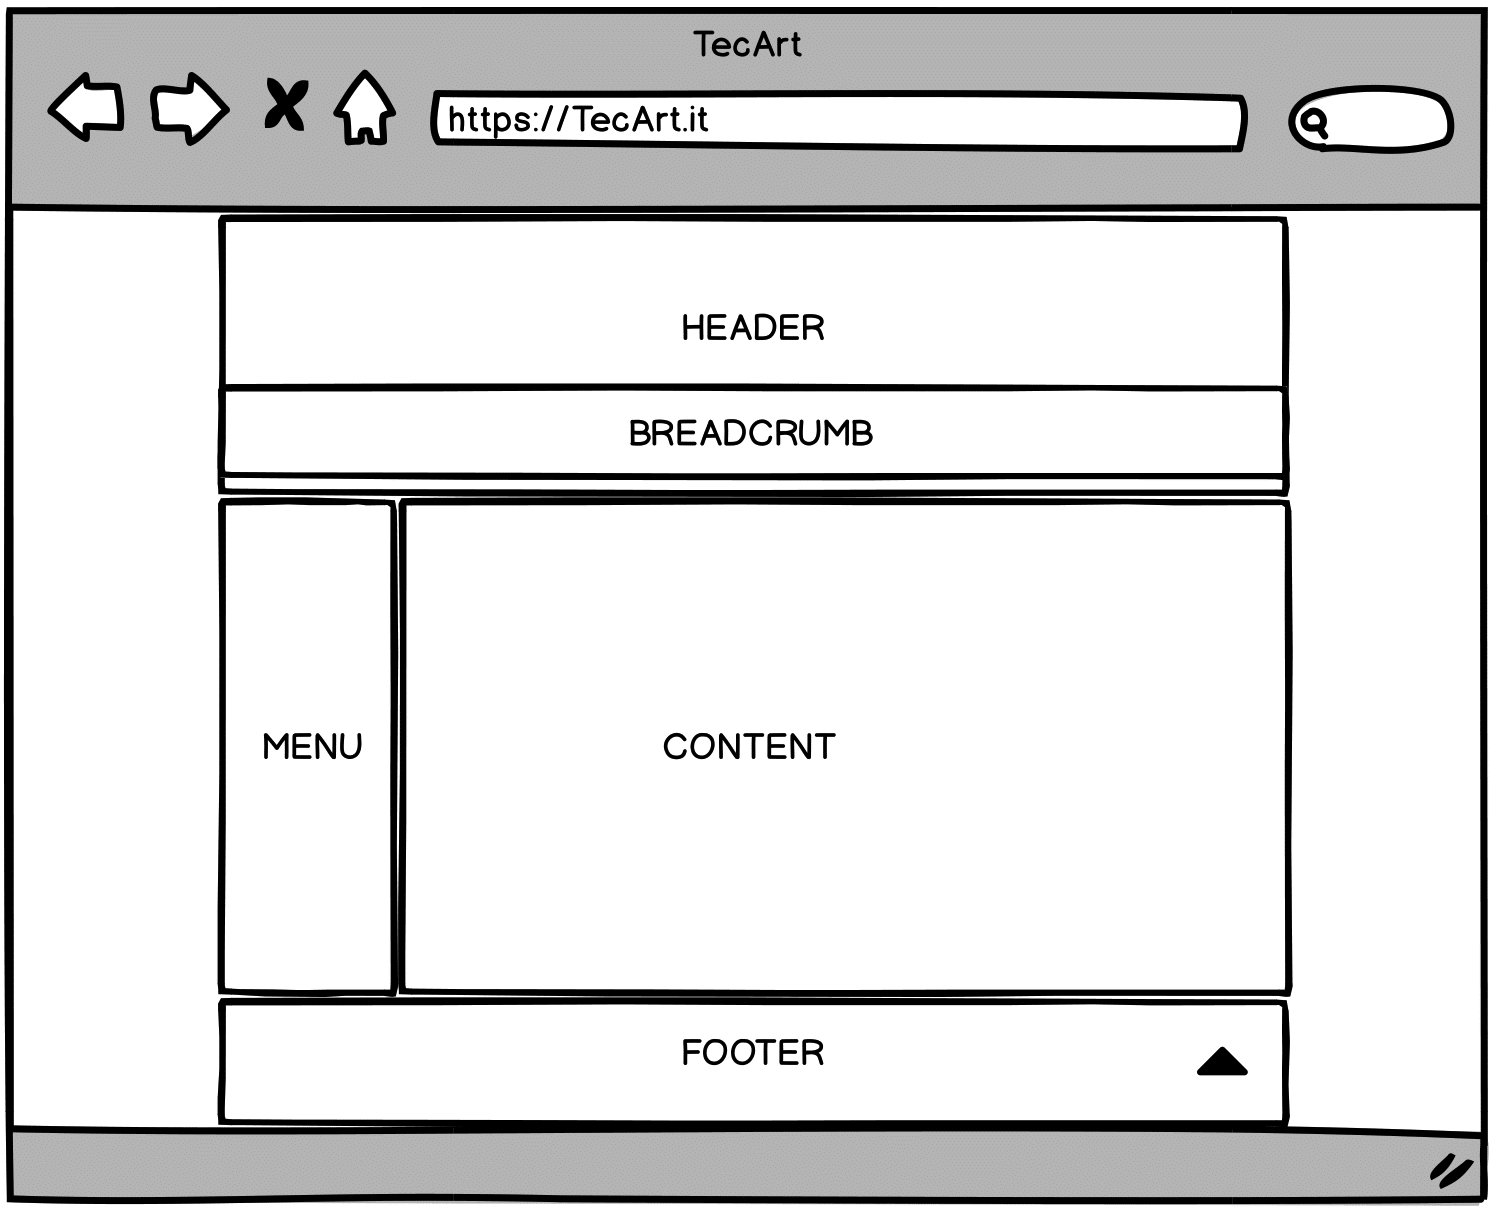
\includegraphics[width=\textwidth]{img/Desktop}
	\captionof{figure}{\textit{Layout desktop}}
\end{center}


\subsection{Accessibilità e usabilità}
\label{progettazione-accessibilità-usabilità}
Sin dalla fase di progettazione ogni aspetto del sito è stato pensato considerando le esigenze di tutte le possibili categorie di utenti. 


A questo scopo, nel rispetto delle specifiche di progetto, il gruppo si è ispirato ai seguenti principi:
\begin{itemize}
	\item \textbf{separazione tra struttura, presentazione e comportamento:} tutte le parti statiche delle pagine sono state implementate in XHTML Strict, la parte di presentazione grafica in CSS3, il comportamento con JavaScript, per i controlli dell'input lato \textit{client}, e PHP7, per i controlli dell'input latoto server, la gestione dei contenuti e l'interazione con database;
	\item \textbf{comprensibilità e navigabilità del sito:} l'organizzazione dei contenuti nelle varie pagine è stata pensata in modo che la struttura fosse coesa e comprensibile all'utente, e che la suddivisione aiutasse il visitatore a trovare tutte le informazioni desiderate nella pagina attesa. 
	\item \textbf{contenuti equivalenti:} gli unici contenuti non testuali presenti nel sito sono le immagini, principalmente quelle delle opere esposte; per ogni figura è stato debitamente definito l'attributo \texttt{alt} del relativo tag HTML, in modo da fornire un'alternativa testuale coerente ed esplicativa del contenuto dell'immagine; in caso di immagini non semanticamente significative, esse sono inserite tramite CSS con la proprietà \texttt{background} (tecnica dell'\textit{image replacement});
	\item \textbf{scelta dello schema colori:} i colori del sito sono stati scelti in modo da non risultare di ostacolo alla consultazione per utenti ipovedenti o affetti da daltonismo; il software usato per i test è \textit{WebAIM} (\url{https://webaim.org/resources/contrastchecker/}); 
	\item \textbf{convenzioni colore per i link:} nel rispetto delle convenzioni più diffuse nei browser, i link risultano blu se mai visitati prima, altrimenti violetto; in ogni caso sono sottolineati. Unica eccezione a queste regole grafiche sono i button contenenti link: in questi casi non si è ritenuto necessario applicare le convenzioni sopra citate perché la forma stessa del button lo rende immediatamente riconoscibile come tale e perfettamente distinguibile dal resto del testo;
	\item \textbf{gestione delle peculiarità dei linguaggi naturali:} per facilitare la sintesi vocale, tutte le parole appartenenti a lingue diverse da quella indicata nell'attributo \texttt{xml:lang} di ogni pagina sono marcate opportunamente in modo da segnalare l'idioma di provenienza. Poichè il sito prevede la possibilità di inserimento di testo da parte degli utenti, autenticati o amministratori, i form di inserimento raccomandano di marcare eventuali termini stranieri con tag creati \textit{ad hoc}: in presenza di questi tag, tramite controlli PHP, al momento dell'inserimento del contenuto nella pagina del sito vengono inseriti i tag HTML corretti, con l'attributo \texttt{lang} impostato correttamente;
	\item \textbf{strutturazione delle pagine a prescindere dalla tecnologia in uso:} l'interfaccia utente è stata studiata in modo da essere intuitiva e di agile navigabilità anche per utenti con disabilità visive. Gli elementi grafici sono stati dimensionati in modo da non essere nè troppo grandi (caratteristica che li renderebbe inadatti alla fruizione tramite \textit{magnifier} o altri strumenti di ingrandimento) nè troppo piccoli (aspetto che renderebbe difficile la navigazione a chiunque non avesse una vista ottima). Si è avuta cura che le scelte di progettazione e grafiche tenessero fossero compatibili anche con le versioni più vecchie dei vari browser, e quando ciò non è stato possibile si è cercato di garantire il più possibile la traformazione elegante (vedi §\ref{implementazione});
	\item \textbf{indipendenza dal dispositivo usato per la navigazione:}
	\item \textbf{guida alla navigazione:}
	\begin{itemize}
		\item \textbf{breadcrumb}: l'utente ha sempre ha disposizione la sequenza ordinata delle pagine visitate per arrivare a quella corrente, così da evitare disorientamento;
		\item \textbf{tabindex:} questo attributo non è stato usato nelle pagine del sito poiché l'ordine del DOM corrispondeva già a quello desiderato per la navigazione;
		\item \textbf{link \texttt{torna su}:} per raggiungere rapidamente l'\textit{header} della pagina (o comunque la sua parte iniziale), senza dover fare scroll verso l'alto;
		\item \textbf{link \texttt{salta al...}:} per gli utenti che non possono usare puntatore o mouse per arrivare rapidamente al contenuto desiderato, sono stati predisposti dei link interni alle pagine per raggiungere direttamente alcuni punti significativi del contenuto (per esempio, evitare tutto lo scorrimento del menu e passare direttamente al corpo della pagina).
	\end{itemize}
\end{itemize}

	\pagebreak
	\section{Implementazione}
\label{implementazione}

\subsection{XHTML}
\label{implementazione-html}
Per la struttura statica delle pagine del sito è stato utilizzato XHTML 1.0 Strict. Si è scelto questo linguaggio perché supportato da gran parte dei browser, anche nelle loro versioni meno recenti, e perché regolato da una sintassi molto rigida, che rende quasi univoca l'interpretazione dei diversi elementi da parte dei browser stessi. È stato scartato HTML5 perché tutte le funzionalità necessarie allo sviluppo del sito erano già offerte da XHTML 1.0 Strict e attualmente non è ancora completamente supportato da tutti i browser per i quali si vuole rendere compatibile il sito.

Il contenuto statico delle pagine è composto da header, breadcrumbs (nella struttura, non sempre nel contenuto), struttura del content e footer.

Per garantire la separazione tra contenuto e presentazione non sono stati usati tag XHTML 1.0 Strict di stile nè è stato inserito codice CSS all'interno dei file \textit{.html}. Si è inoltre evitato di inserire tag XHTML 1.0 Strict strutturali col solo scopo di usarli come base per le regole CSS. 

\subsubsection{Strumenti}
\label{implementazione-html-strumenti}

\paragraph{w3schools HTML reference}
\label{implementazione-html-strumenti-w3schools-reference}
Per valutare la compatibilità dei tag utilizzati rispetto ai vari browser, anche nelle loro versioni meno recenti, ci si è affidati al sito di \textit{w3schools}, che riporta, per ogni tag XHTML 1.0 Strict, le informazioni di compatibilità.


\subsection{CSS}
\label{implementazione-css}
Per la presentazione grafica del sito è stato utilizzato CSS3. Nella scelta delle regole CSS si è cercato di garantire l'accessibilità ad utenti affetti da disabilità visive non completamente invalidanti e di evitare effetti grafici che avrebbero potuto causare disagio ad utenti affetti da disturbi comportamentali.

\subsubsection{Strumenti}
\label{implementazione-css-strumenti}

\paragraph{w3schools CSS reference}
\label{implementazione-css-strumenti-w3schools-reference}
Per valutare la compatibilità delle regole utilizzate rispetto ai vari browser, anche nelle loro versioni meno recenti, ci si è affidati al sito di \textit{w3schools}, che riporta, per ogni regola CSS, le informazioni di compatibilità.

\subsection{PHP}
\label{implementazione-php}
Per i controlli sull'input lato server e le interazioni col database è stato usato PHP7. Nonostante tutti i controlli lato client siano fatti in linguaggio JavaScript, è necessario effettuarli anche lato server qualora i primi falliscano, ad esempio se JavaScript è disabilitato. L'uso di PHP ha permesso anche di diversificare il comportamento dinamico delle pagine, a seconda dei risultati ottenuti dalle operazioni col database e del tipo di utente (generico, autenticato o amministratore) che interagisce col sito. In questo modo, infatti, si ottiene la completa separazione del comportamento dal contenuto e dalla presentazione.

Il file \textit{.php} sono stati divisi in \textit{Database}, \textit{Repository}, \textit{Controller}, \textit{Utilities} e [NomePagina].php. 
\begin{itemize}
	\item \textbf{Database:} un singolo file chiamato DatabaseAccess.php offre metodi per la preparazione e l'esecuzione di query al database differenziando quelle che fanno uso dello select statement da quelle prive di esso;
	\item \textbf{\textit{Repository}:} uno per ogni tabella del database, offre metodi per l'esecuzione di query sulla rispettiva tabella, che implementano le operazioni \textit{CRUD:} inserimento, lettura, modifica e cancellazione. Di queste sono fornite numerose versioni al fine di implementare le funzionalità in modo soddisfacente. Per la tabelle Opere sono offerti due tipi di contenuto diversi, dipinti e sculture, che però, a differenza delle due tipologie di evento, necessitano di campi dati distinti. Dunque si sono costruite query diversificate per risolvere questa evenienza;
	\item \textbf{\textit{Controller}:} invocano i metodi esposti dalle \textit{Repository} mettendo in comunicazione le pagine [NomePagina].php col database.
	In particolare forniscono un'interfaccia per trasformare i dati dal formato predisposto all'utente, pagine [NomePagina].php, a quello utilizzato dal database, \textit{Repository}, e viceversa. Offrono inoltre tutti i metodi per eseguire i controlli sull'input dell'utente: alcuni controlli generici (trim per l'eliminazione degli spazi bianchi in testa ed in coda, sostituzione dei caratteri speciali con le apposite \textit{entity}, eliminazione dei possibili tag XHTML o comandi PHP e gestione delle parole in lingua straniera con opportuni tag come [en][/en]) sono comuni a tutti i controller, altri invece sono specifici del contenuto che gestiscono.
	\item \textbf{\textit{Utilities}:} il file DateUtilities.php gestisce le conversioni del formato di data; il file FileUtilities.php effettua i controlli sul caricamento dei file da parte dell'utente, poiché l'inserimento di un'opera nel sito richiede anche il caricamento di un'immagine; mentre DataUtilities.php contiene solo funzioni statiche, FileUtilities.php ne è composto solo in parte;
	\item \textbf{[NomePagina].php:} una per ogni pagina \textit{.html} statica, gestisce il caricamento dei contenuti dinamici del sito e la loro organizzazione nella pagina, la gestione delle connessioni al database, la chiamata delle funzioni per l'interazione tra pagina e database delegando il compito controller e le funzionalità a disposizione a seconda del tipo di utente che sta navigando il sito.
\end{itemize}
Grazie a questa suddivisione il codice risulta molto più leggibile e di facile debug oltre ad evidenziare una separazione tra ciò che viene visualizzato all'utente e i dati che invece sono salvati.

\subsubsection{Sessioni}
\label{implementazione-php-sessioni}
Per memorizzare alcune informazioni nel passaggio da una pagina all'altra sono state usate le sessioni. Più precisamente, si tiene traccia dello username dell'utente e della sua tipologia (admin, autenticato, non autenticato), della paginazione dei contenuti (se si tratta di pagine che coinvolgono gli elenchi di opere, eventi, recensioni o utenti) e altri parametri simili necessari a mantenere le informazioni essenziali ad un'ottimale esperienza d'suo dell'utente durante l'intera navigazione.

Per gestire adeguatamente il caso in cui un utente conservasse il bookmark di una pagina richiedente specifici parametri di sessione per essere acceduta, si è deciso di prevedere un'impostazione di default dei parametri stessi in assenza del passaggio di valori effettivi. In questo modo sarà comunque possibile accedere alla pagina salvata ed interagire con essa e col breadcrumbs senza rischio di errori.

\subsection{JavaScript}
\label{implementazione-javascript}
Il linguaggio Javascript è stato usato principalmente per i controlli sull'input lato client: nonostante infatti i controlli siano comunque effettuati lato server (vedi §\ref{implementazione-php}), poiché le elaborazioni \textit{server side} sono più lente e onerose, è preferibile effettuare più controlli possibile direttamente lato client, e fermare lì eventuali input errati. Per questo motivo le operazioni effettuate dai metodi JavaScript per controllare l'input sono analoghe a quelle dei corrispondenti metodi PHP lato server.

Lo script JavaScript usato è unico e contiene tutti i metodi per il controllo e la gestione degli input, differenziati per opera, evento, recensione, utente e risultato della ricerca.

Per tutti i form si controlla l'appropriatezza dei dati inseriti dall'utente: se sono errati, sopra il campo di input viene mostrato un messaggio di errore, spesso associato ad un suggerimento sul tipo di errore commesso \footnote{Per agevolare ancora di più l'utente nella compilazione dei form, sono previsti dei suggerimenti associati ai campi a completamento meno intuitvo; questi suggerimenti sono statici, inseriti quindi in XHTML 1.0 Strict.}

Oltre al controllo degli input e segnalazione degli errori, JavaScript gestisce le funzionalità:
\begin{itemize}
	\item il menu ad hamburger a comparsa, per il layout mobile;
	\item la rimozione della mappa dalla pagina dei \textit{Contatti} se visualizzata da browser \textit{Internet Explorer 9} e \textit{Internet Explorer 10}, perché non supportato; questo non diminuisce la comprensibilità delle informazioni fornite, poiché la mappa è comunque corredata da indicazioni stradali scritte;
	\item la selezione dello stile dell'opera per abilitare correttamente i campi in fase di inserimento e modifica;
	\item i filtri per la visualizzazione di contenuti;
	\item visualizzazione dell'anteprima dell'immagine inserita per le opere.
\end{itemize}


È stato possibile implementare in JavaScript tutti i controlli previsti in PHP; unica eccezione il controllo sulla dimensione dell'immagine caricata via browser \textit{Internet Explorer 9}, per problemi di sopporto dei metodi; si è comunque avuto cura di raffinare il più possibile il controllo su questo tipo di input, in modo da ridurre al minimo il numero di invii scorretti verso al server.

Si è deciso di non adottare JQuery per la risoluzione di questo problema di compatibilità per evitare di appesantire il sito, trattandosi questo di un unico caso di controllo incompleto lato client.


\subsubsection{Strumenti}
\label{implementazione-javascript-strumenti}

\paragraph{MDN web docs}
\label{implementazione-javascript-strumenti-mdn}
Per valutare la compatibilità dei meotodi utilizzati rispetto ai vari browser, anche nelle loro versioni meno recenti, ci si è affidati al sito di \textit{MDN} (\url{https://developer.mozilla.org/it/docs/Web/JavaScript}), che riporta, per ogni metodo, le informazioni di compatibilità.


	\pagebreak
	\section{Presentazione}
\label{presentazione}
Nel definire la grafica del sito si è partiti dall'interfaccia mobile, per poi fissare ulteriori regole per gli elementi il cui aspetto doveva adattarsi a finestre più grandi. Questo si vede dalla struttura del foglio di stile \textit{Style.css}: le regole iniziali sono proprie del formato mobile, se possibile applicate anche agli altri formati; seguono le regole del formato tablet, racchiuse in un'apposita media query; infine quelle per il desktop, anch'esse in una media query. I vantaggi dell'approccio mobile first sono:
\begin{itemize}
	\item molti utenti navigano da dispositivi mobili, quindi è importante curare l'esperienza di navigazione in schermi piccoli, in particolare la grafica;
	
	\item partire dal dispositivo più piccolo va incontro al principio di responsive design (design che si adatti alle dimensioni della finestra del browser): è più facile partire da una schermata piccola e poi ingrandirla, includendo mano a mano più elementi, rispetto all'approccio inverso, che rischia, nel passaggio dal grande al piccolo,  di comprimere le informazioni in spazi troppo stretti;
	
	\item una grafica che parta dal mobile si concentra da subito sugli elementi fondamentali delle pagine, poiché deve sfruttare al meglio lo spazio a disposizione: ciò è un vantaggio nel successivo design delle finestre più ampie.
\end{itemize}

Il foglio di stile per la grafica da schermo è unico per tutti i formati, in modo da ottimizzare al massimo il codice. Allo stile di stampa è stato dedicato un secondo file, poiché molti elementi visualizzati a schermo sono eliminati dal formato di stampa, e aspetti basilari, come il font o i margini, sono diversi tra stampa e display.

\subsection{Mobile}
\label{presentazione-mobile}

\begin{center}
	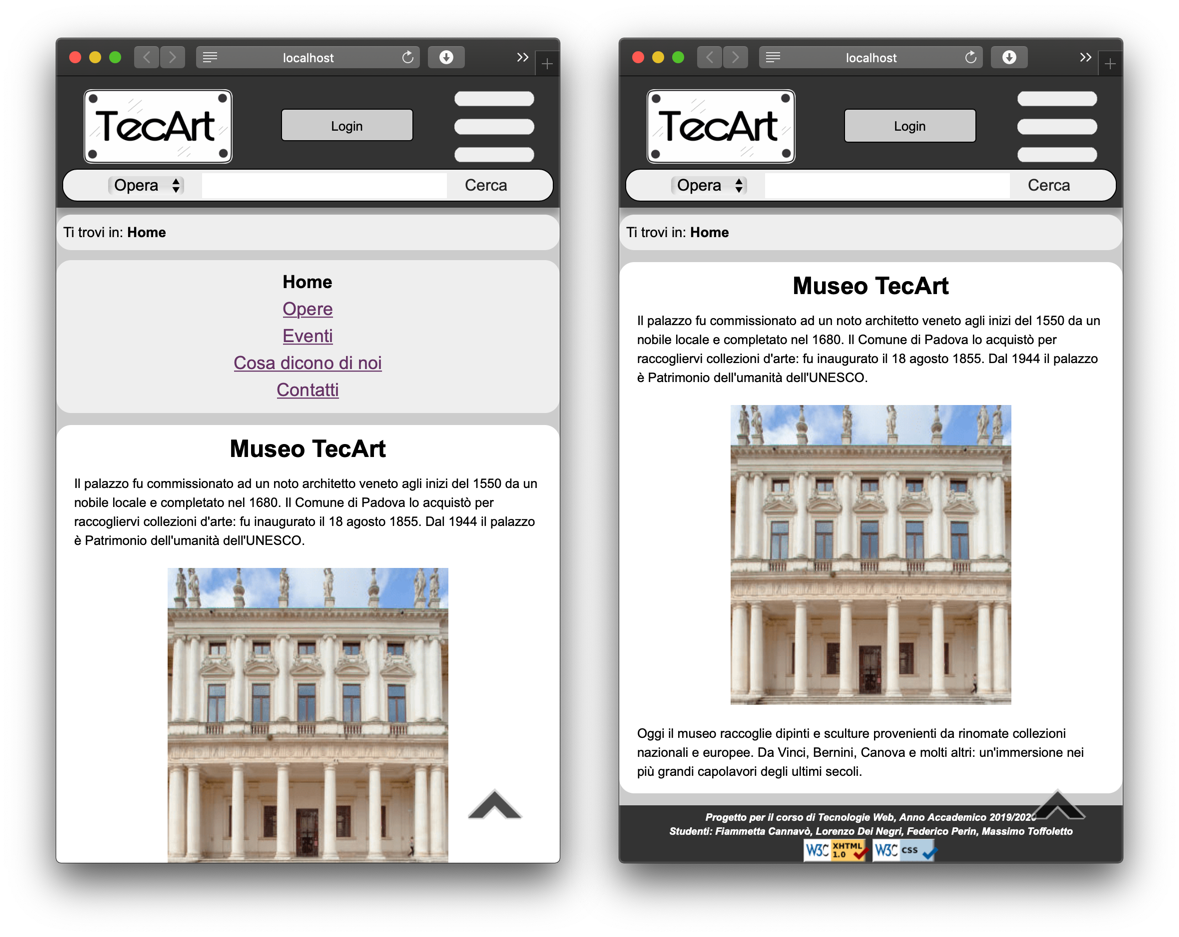
\includegraphics[scale=0.27]{img/Mobile-pres}
	\captionof{figure}{Grafica mobile con menu visibile (a sinistra) e nascosto (a destra)}
\end{center}

La grafica mobile presenta un header contenente logo, menu per il login e la gestione dell'area personale e l'icona per il menu ad hamburger. Per il menu è stata scelta un'icona, invece di un button contenente del testo, perché più coerente con la grafica adottata per le interfacce \textit{mobile}. Segue il breadcrumb e subito sotto il corpo della pagina. In fondo alla schermata si trovanp il footer e la freccia per tornare all'inzio della pagina senza scroll verticale. Cliccando sull'icona ad hamburger, sotto il breadcrumb compare il menu, altrimenti non visualizzabile. Si è deciso di nascondere il menu del sito per evitare di occupare la schermata, già piccola, con contenuti diversi dal corpo della pagina.

\subsection{Tablet}
\label{presentazione-tablet}

\begin{center}
	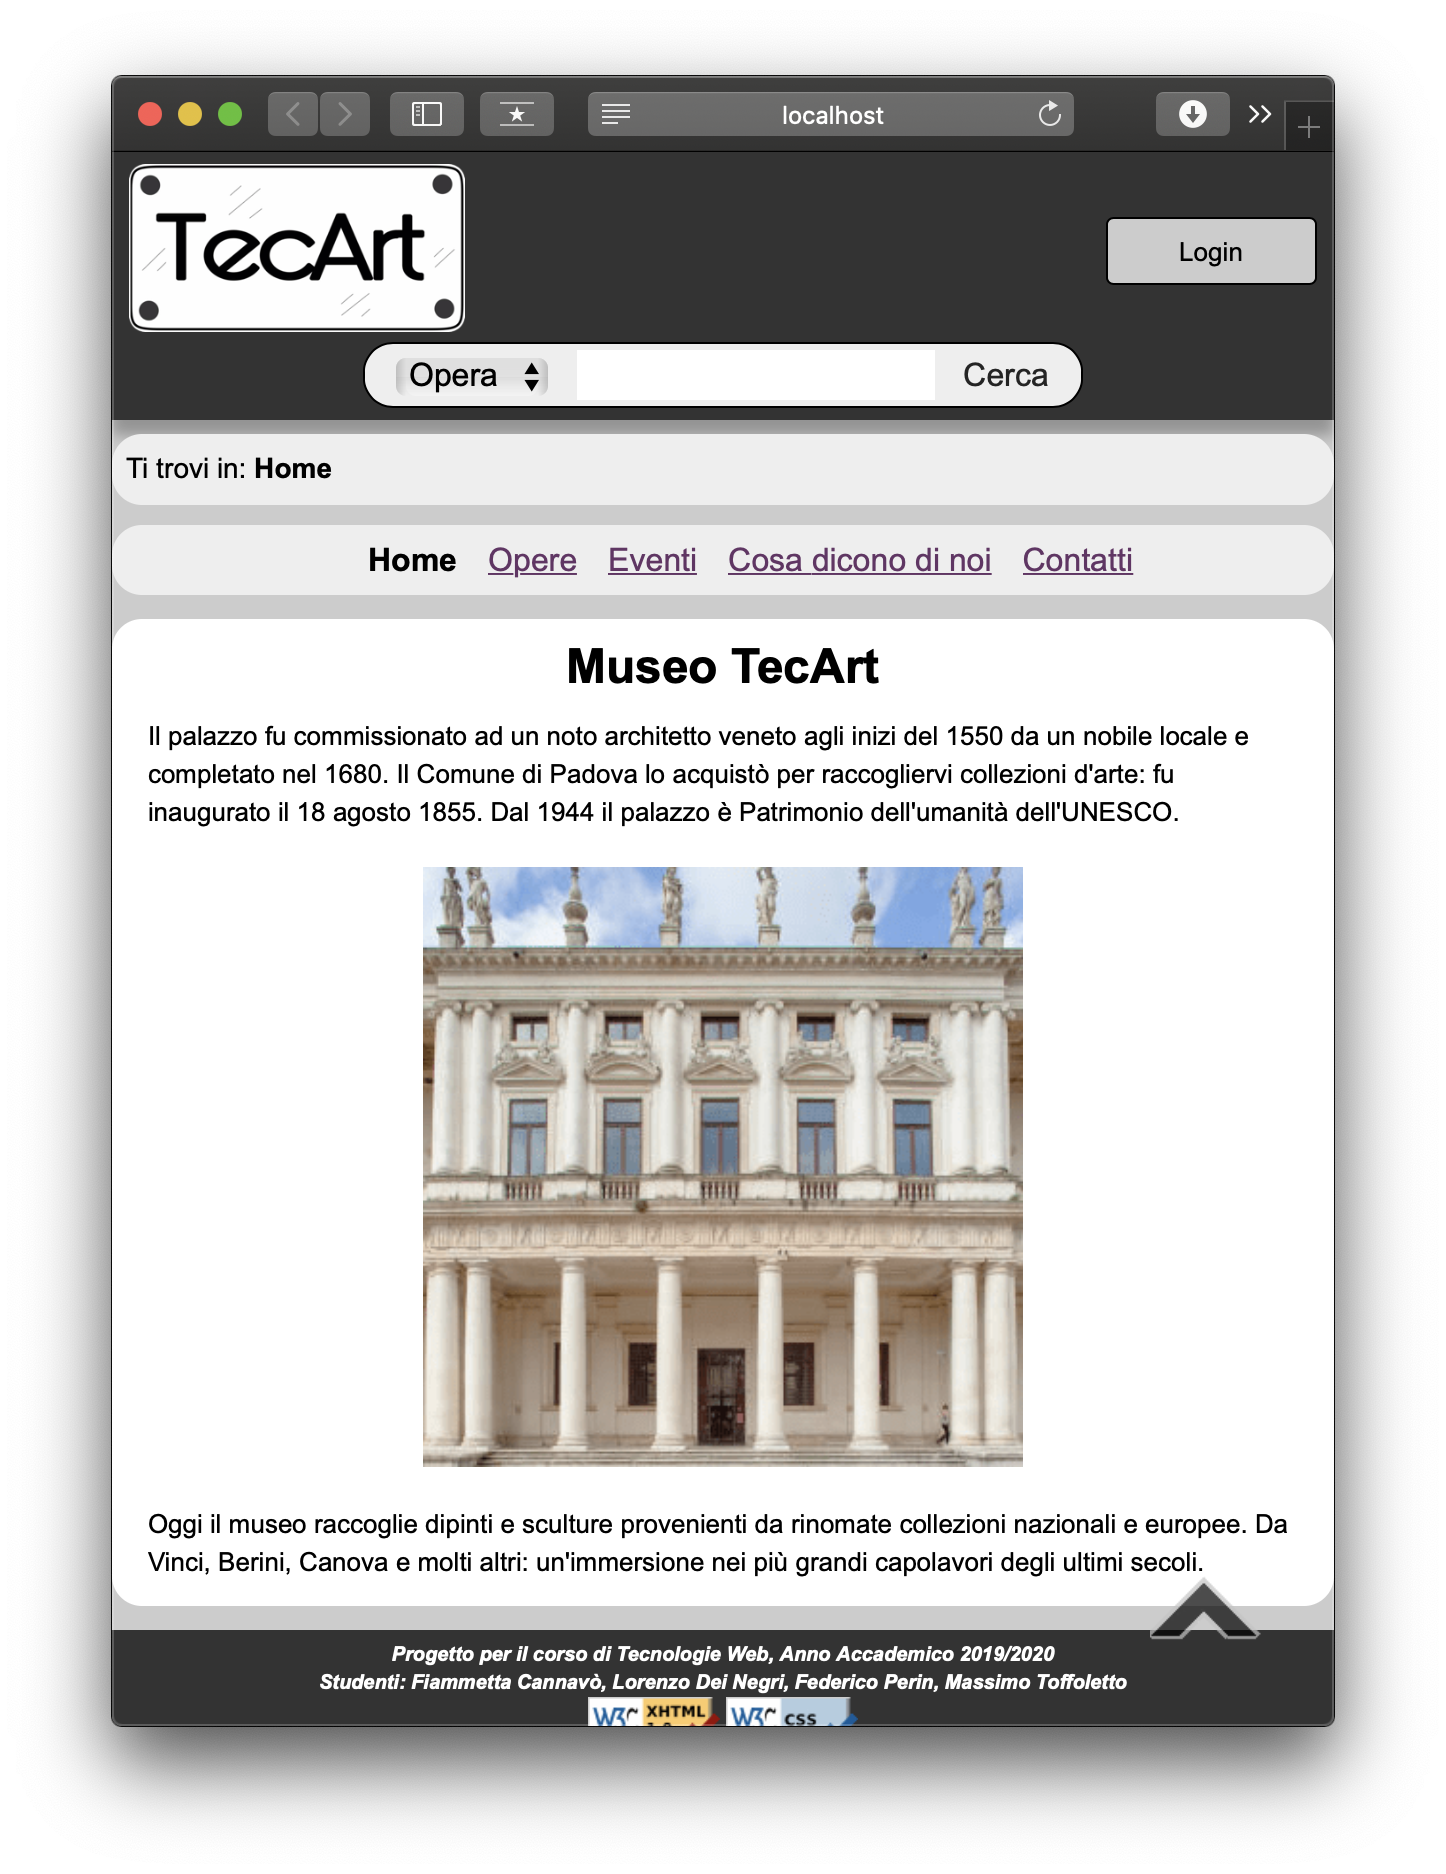
\includegraphics[scale=0.45]{img/Tablet-pres}
	\captionof{figure}{Grafica tablet}
\end{center}

La peculiarità del formato tablet è la posizione del menu: scompare l'icona ad hamburger e il menu è spostato sotto il breadcrumb. I link non sono più incolonnati ma posti in un'unica riga: in questo modo si evita di rubare troppo spazio al corpo della pagina, ma allo stesso tempo, essendo la schermata più ampia rispetto a quella di uno smartphone, si evita che l'utente debba effettuare un click per visualizzare il menu.


\subsection{Desktop}
\label{presentazione-desktop}

\begin{center}
	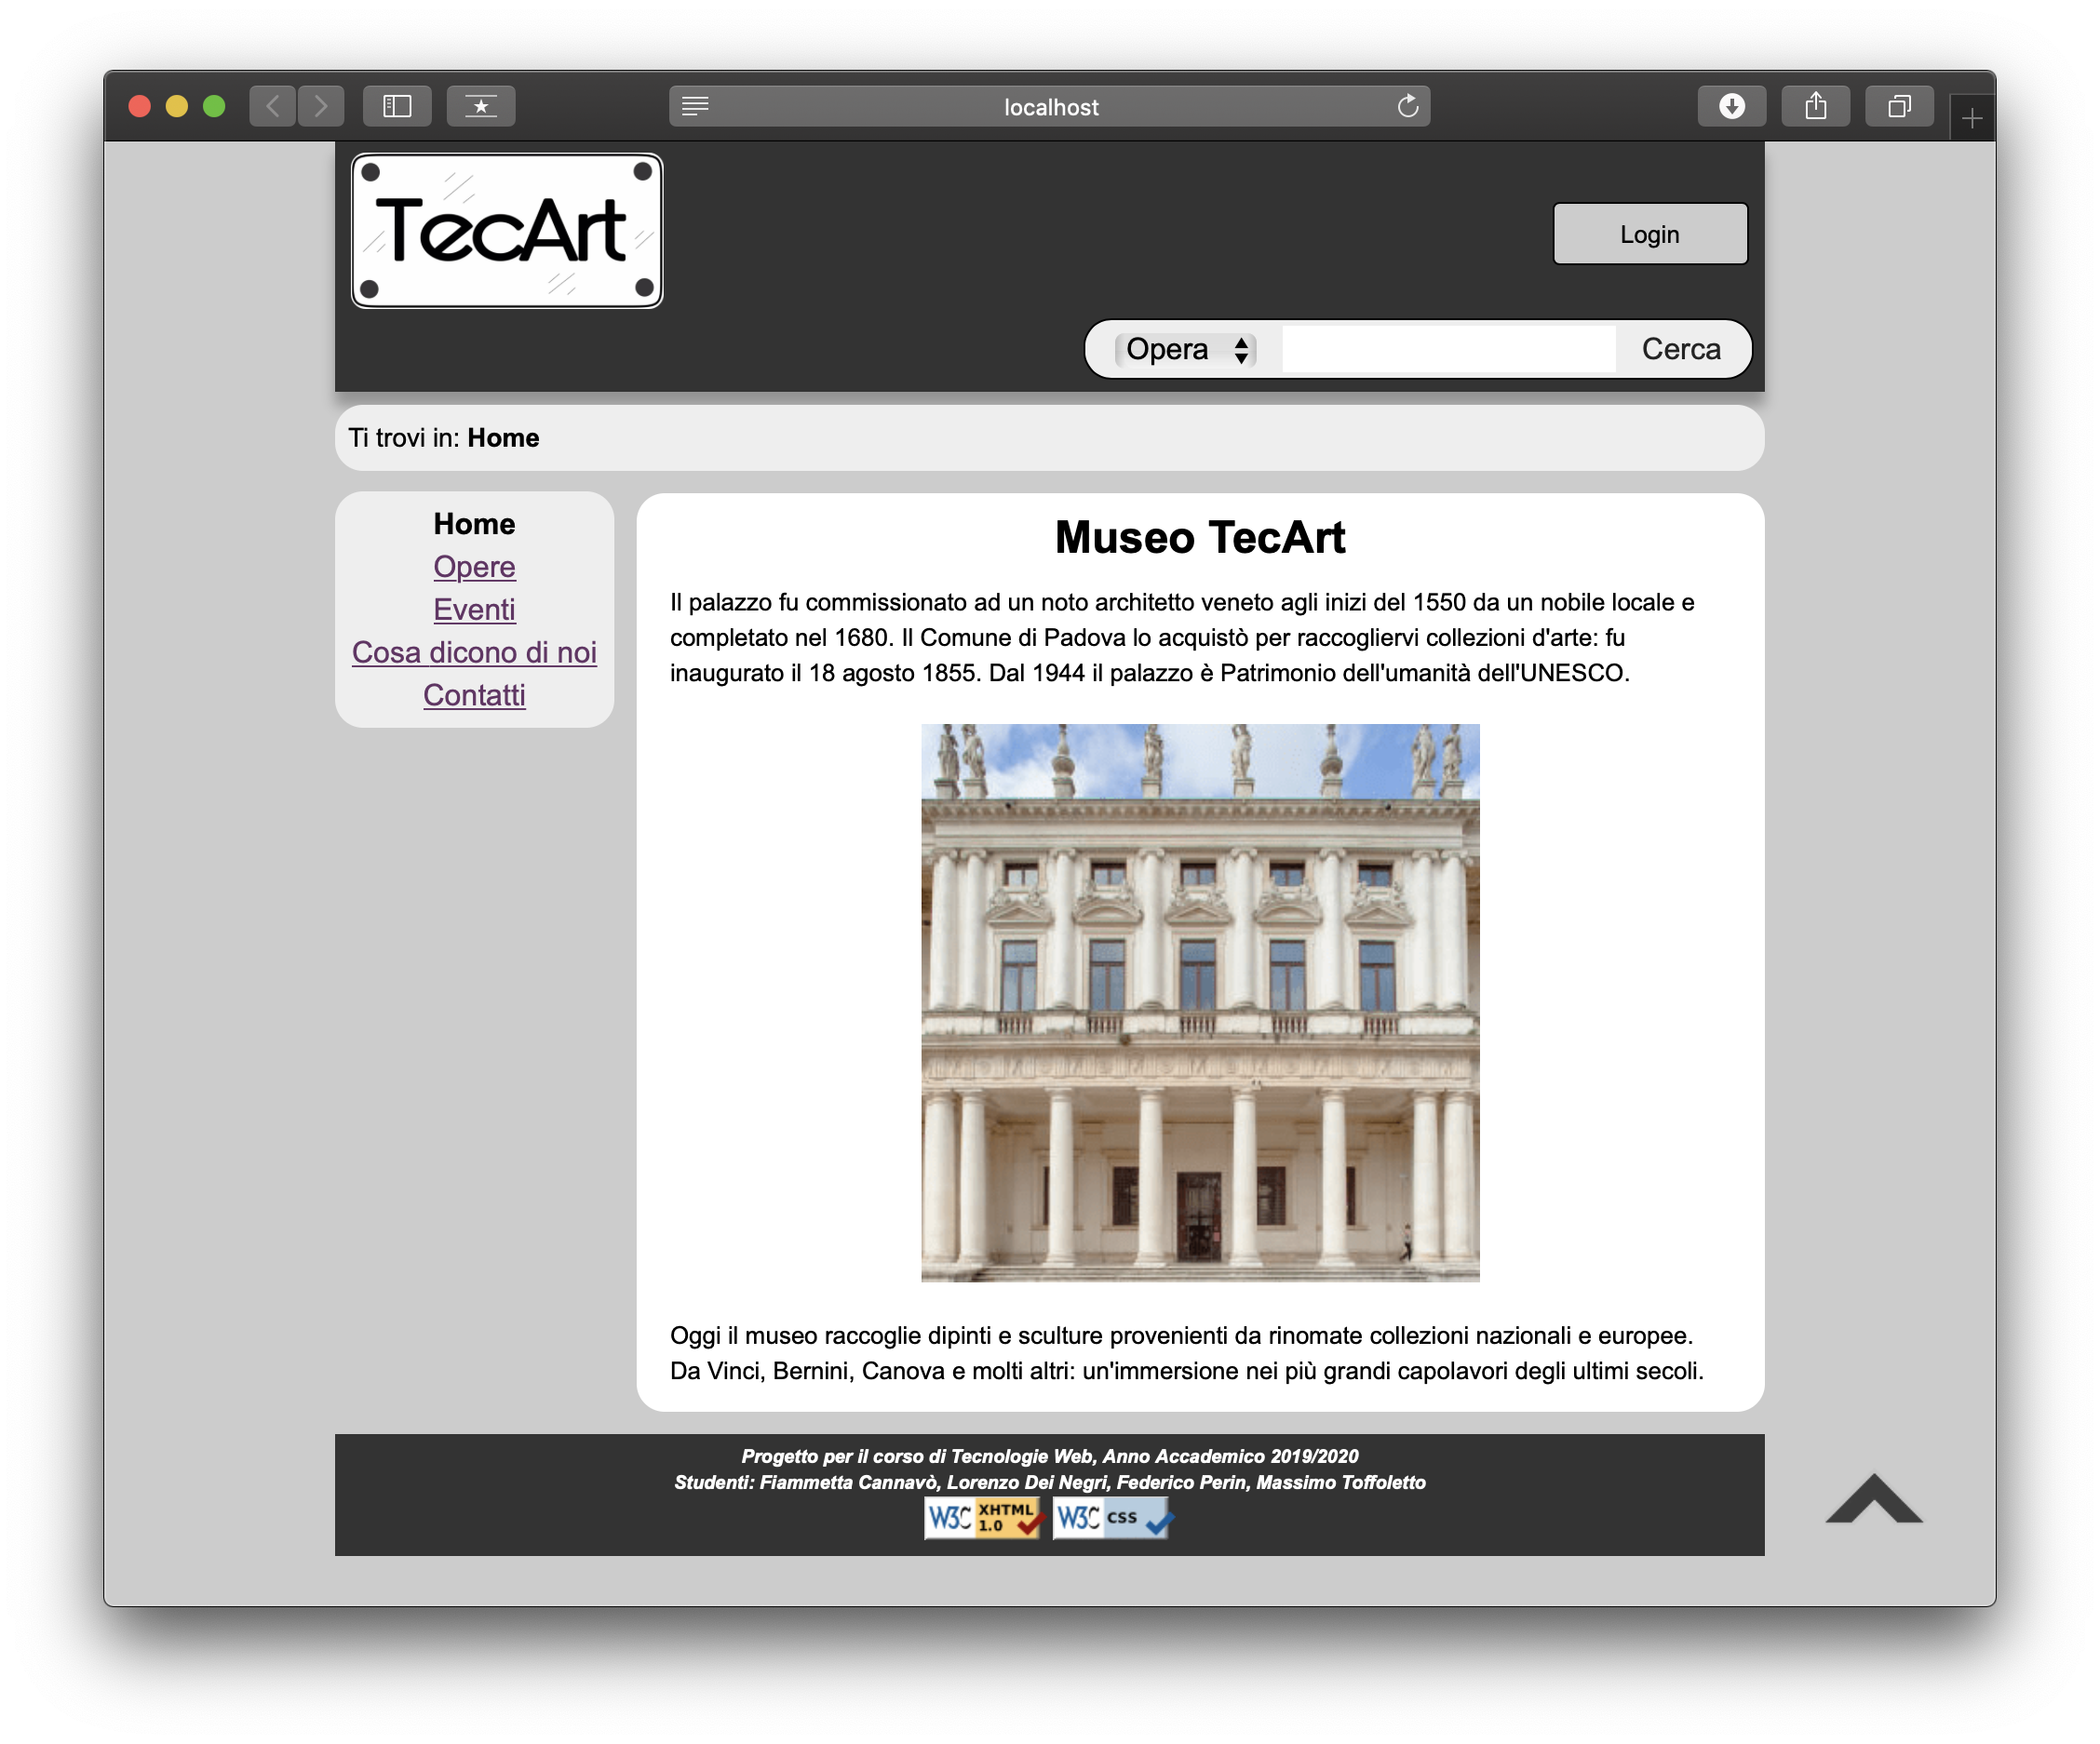
\includegraphics[width=\textwidth]{img/Desktop-pres}
	\captionof{figure}{Grafica desktop}
\end{center}
Ancora una volta, a cambiare è l'aspetto del menu: avendo a disposizione una finestra ampia è possibile mantenere il menu sempre a schermo, posizionandolo però sul lato sinistro, in modo da lasciare più spazio possibile, in verticale, al contenuto della pagina. Per garantire un'esperienza positiva di navigazione anche agli utenti con uno schermo piccolo, si è deciso di limitare l'ampiezza massima della finestra a 1024px, eventualmente occupando il resto della finestra con uno sfondo uniforme, in liena con la palette di colori del sito.


\subsection{Stampa}
\label{presentazione-stampa}

%\begin{center}
%	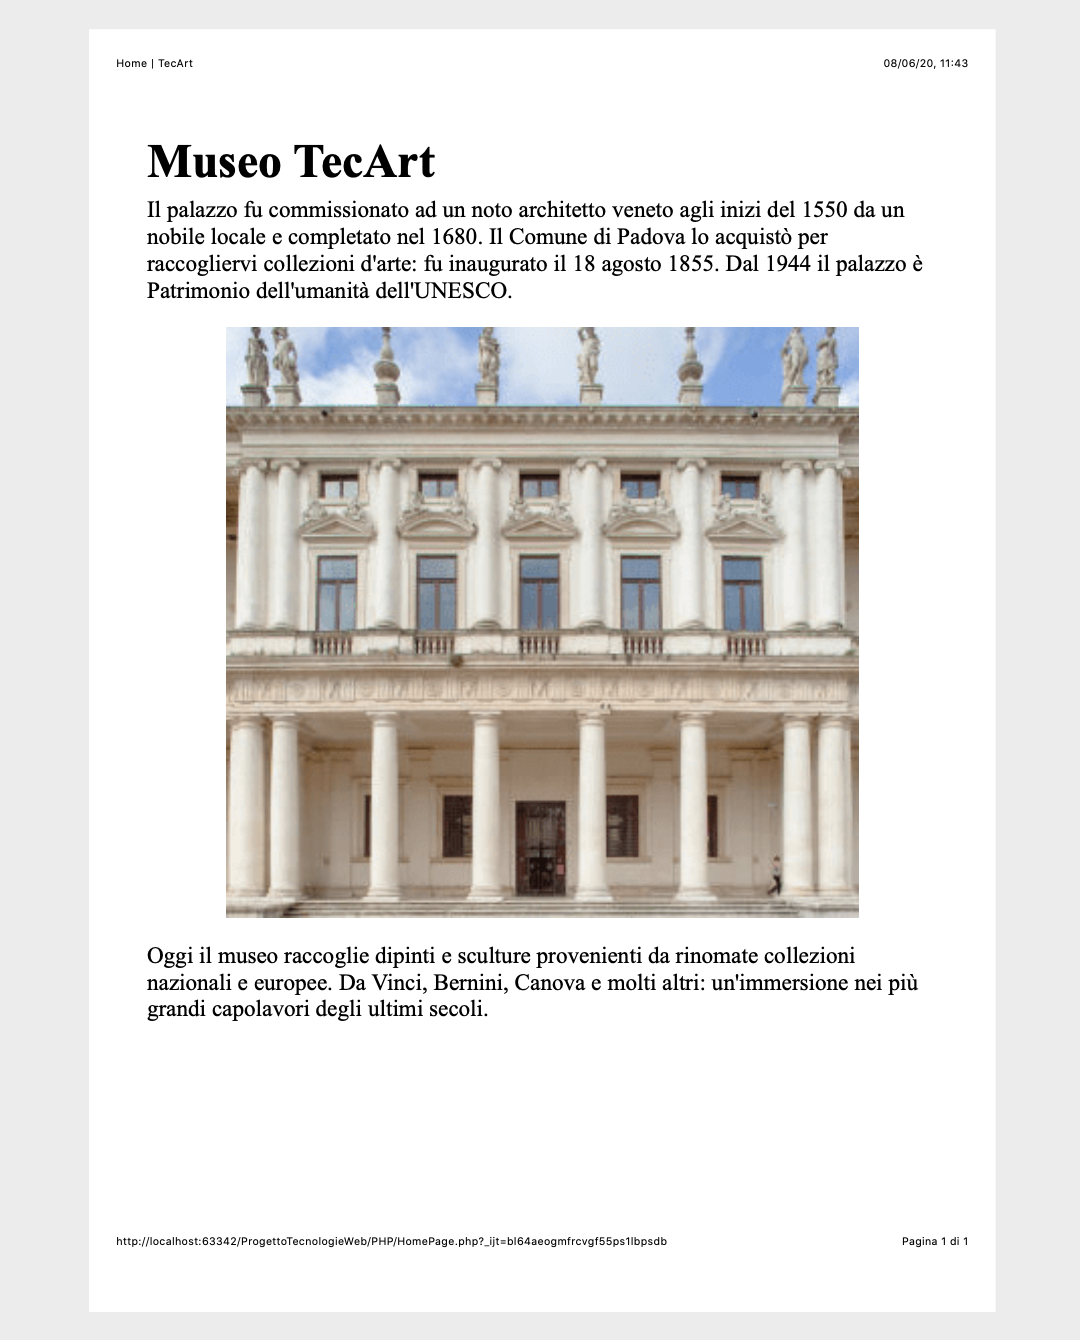
\includegraphics[scale=0.16]{img/Stampa-pres}
%	\captionof{figure}{Grafica stampa}
%\end{center}

Il layout di stampa omette tutti i sopporti alla navigazione: non compaiono i menu, il breadcrumb e i button. Sono rimosse anche tutte le immagini non significative, anche se si è ritenuto opportuno mantenere quelle delle opere, trattandosi del sito di un museo di opere d'arte. Tutto questo si vede dalla struttura del foglio di stile \textit{Print.css}.

	\pagebreak
	\section{Validazione}
\label{validazione}

\subsection{Obiettivi}
\label{validazione-obiettivi}

In vari momenti, durante lo sviluppo del sito, parte del codice prodotto è stato sottoposto a validazione tramite strumenti autorevoli (vedi §\ref{validazione-strumenti}). La validazione è un'attività fondamentale per la creazione di un sito web di qualità e ben fatto. Innanzitutto, un codice valido funziona esattamente secondo le specifiche del linguaggio cui appartiene, senza comportamenti anomali o imprevisti, cosa invece frequente quando si ha a che fare con codice non valido. 

Inoltre, il rispetto delle regole di validazione garantisce un rating migliore del sito al momento dell'indicizzazione da parte dei diversi motori di ricerca: questo comporterebbe un posizionamento più in basso tra i risultati delle ricerche, con una conseguente penalizzazione nel numero di accessi al sito.

In ottica di massima navigabilità e portabilità del sito, il codice valido è generalmente più compatibile con i numerosi browser attualmente in uso; risulta anche più semplice controllare il comportamento e la presentazione del sito su browser diversi, oltre che a garantire la compatibilità con essi dei costrutti usati.

Infine, tutte le categorie di utenti impossibilitate a navigare il sito con un computer fornito di schermo e puntatore, o affetti da disabilità di vario genere, sarebbero penalizzate, perché gli strumenti da essi adottati (per esempio, i lettori di schermo) faticano ad interpretare correttamente codice con errori di validazione.


\subsection{Strumenti}
\label{validazione-strumenti}

Per i controlli di validazione delle pagine del sito sono stati usati due strumenti:
\begin{itemize}
	\item \textbf{W3C Markup Validation Service}, per la validazione delle pagine scritte in XHTML. Il controllo di conformità alle regole del W3C è stato fatto in due fasi. Inizialmente sono state validate tutte le pagine statiche, sottoponendo allo strumento il codice XHTML statico. In un secondo momento, con l'aggiunta del codice PHP, sono state validate le pagine complete del sito, composte da codice XHTML sia statico che aggiunto dinamicamente tramite PHP. Il codice delle singole pagine veniva prelevato grazie agli strumenti di sviluppatore messi a disposizione dai vari browser, principalmente \textit{Firefox}, \textit{Google Chrome} e \textit{Safari}, e sottoposte ai controlli del validatore. La prima fase di validazione ha permesso di correggere sin da subito alcuni errori, in modo che, durante la seconda fase, fossero presenti solo eventuali imprecisioni legate al codice XHTML aggiunto dinamicamente. Lo strumento permette di validare sia per inserimento di URI, sia per upload di file, sia per input diretto del codice: quest'ultima modalità è stata la più adottata. Il validatore segnala gli errori in maniera puntuale e precisa, dando dei suggerimenti di correzione, in modo che la loro individuazione e risoluzione sia rapida. Il servizio è reperibile gratuitamente al link: \url{https://validator.w3.org}.
	
	\item \textbf{W3C CSS Validation Service}, per la validazione del codice CSS. Il controllo di conformità dei fogli di stile è stato meno complicato rispetto a quello delle pagine XHTML, poichè il codice era meno lungo e raggruppato in soli due file, uno dedicato alla grafica a schermo e uno a quella a stampa. Le modalità di input del codice e di segnalazione degli errori sono analoghe a quanto detto per il \textit{W3C Markup Validation Service} descritto sopra. Il servizio è reperibile gratuitamente al seguente link: \url{https://jigsaw.w3.org/css-validator/}.
\end{itemize}
	\pagebreak
	\section{Test}
\label{test}
L'attività conclusiva del progetto è stata la verifica del funzionamento del sito. Il testing si è concentrato su due aspetti, spesso strettamente legati: 
\begin{itemize}
	\item funzionamento del sito e delle interazioni col database, efficacia dei controlli dinamici, efficienza del codice;
	\item esperienza e qualità della navigazione, compatibilità con le varie tecnologie, accessibilità e usabilità.
\end{itemize}
Quando possibile, nuove funzionalità e controlli dinamici sono stati testati parallelamente alla loro implementazione, in modo da rendere più rapida la rilevazione degli errori e la loro correzione. Tuttavia, ciò non è stato sempre possibile, quindi buona parte dell'attività di test è stata svolta al termine della codifica.

\subsection{Strumenti}
\label{test-strumenti}

\subsubsection{Strumenti sviluppatore}
\label{test-strumenti-sviluppatore}
Durante i test di funzionamento del sito sono stati usati gli strumenti sviluppatore messi a disposizione dai browser \textit{Mozilla Fireforx}, \textit{Safari}, \textit{Google Chrome}, \textit{Microsoft Edge}. Si sono rivelati molto utili soprattutto al momento della verifica delle pagine dinamiche, in particolare quelle coinvolte nei controlli JavaScript, nelle quali eventuali bug potevano derivare da combinazioni diverse di parti di codice assemblate al momento.

Sono state usate anche le funzionalità di disabilitazione delle immagini o dei colori, in particolare quelli di \textit{Mozilla Fireforx}.


\subsubsection{Lighthouse}
\label{test-strumenti-lighthouse}
\textit{Lighthouse} è uno strumento \textit{open source} automatizzato, eseguibile su qualsiasi pagina web. Offre \textit{audit} per prestazioni, accessibilità, \textit{progressive web app} (non di nostro interesse), \textit{Search Engine Optimization} (SEO) e altro.

I controlli possono essere eseguiti direttamente dagli strumenti sviluppatore offerti da \textit{Google Chrome} o da riga di comando. Dato in input l'URL della pagina, \textit{Lightouse} esegue i controlli e genera un resoconto, contenente consigli migliorativi. 


\subsubsection{XAMPP e MAMP}
\label{test-strumenti-xampp-mamp}
Link per il download: \url{https://www.apachefriends.org/it/download.html}



\subsubsection{Browsershots}
\label{test-strumenti-browsershots}
Link: \url{http://browsershots.org}. 

Browsershots è un'applicazione web che simula un sito web su diversi sistemi operativi e browser. Il servizio è gratuito e permette di verificare il funzionamento delle pagine su un vasto numero di piattaforme diverse, per valutarne compatibilità, funzionamento e accessibilità. I browser di interesse per il sito sono \textit{Mozialla Firefox}, \textit{Google Chrome}, \textit{Safari}, \textit{Microsoft Edge}, \textit{Opera} e \textit{Internet Explorer} 9.

\subsubsection{WAVE}
\label{test-strumenti-wave}
Link: \url{https://wave.webaim.org}.

\textit{Web Accessibility Evaluation tool} (WAVE) è una suite di strumenti di valutazione che permette di migliorere l'accessibilità dei contenuti web. È in grado di identificare molti errori relativi all'accessibilità e allo standard WCAG, ma facilita anche la valutazione umana dei contenuti web.

È possibile usare WAVE online inserendo l'URL di una pagina nel campo apposito. Le estensioni WAVE di \textit{Mozilla Firefox} e \textit{Google Chrome} sono disponibili per testare l'accessibilità direttamente nel browser, utile per controllare pagine protette da password o altamente dinamiche. 


\subsubsection{Silktide}
\label{test-strumenti-silktide}
È un \textit{plugin} gratuito di \textit{Google Chrome} che permette valutare l'accessibilità del sito. Fornisce un resoconto generale del livello di accessibilità, valutando la conformità con lo standard WCAG 2.1. Consente inoltre di navigare il sito simulando le condizioni di utenti affetti da diversi tipi di disabilità, sia visive che comportamentali. 


\subsubsection{NVDA}
\label{test-strumenti-nvda}
Link per il download: \url{https://www.nvda.it/download}.

\textit{Non Visual Desktop Access} (NVDA) è un software \textit{open source} da utilizzabile nei sistemi operativi \textit{Windows7}, \textit{Windows8} e \textit{Windows10}.
Gli utenti affetti da disabilità visive, mediante questo strumento, possono usare un computer in completa autonomia. NVDA è un prodotto gratuito e permette all'utente di conoscere ciò che avviene sullo schermo tramite grazie ad una sintesi vocale.

\subsubsection{Links2}
\label{test-strumenti-links2}
Link per il download: \url{http://links.twibright.com/download.php}.

\textit{Links} è un browser unicamente testuale da linea di comando: permette di navigare le pagine web fruendole unicamente come testo, senza alcuna interfaccia grafica. Questo strumento simula l'impossibilità di accedere alle agevolazioni date dalla grafica, oltre a rappresentare tutta l'utenza che effettivamente non ha gli strumenti per accedere al web in modo diverso dal testo.


	\pagebreak
	\section{Suddivisione del lavoro}
\label{suddivisione-del-lavoro}
Lo sviluppo del sito web è stato possibile solo grazie al lavoro coordinato e sinergico di tutti gli elementi del gruppo. Di comune accordo i membri hanno cercato di lavorare tutti, per quanto possibile, ad ogni aspetto del sito, in modo da rendere il lavoro più equo e acquisire tutti le competenze relative alle varie attività. 
\\Di seguito sono riportate le attività svolte da ciascun componente.  
\begin{itemize}
	\item \textbf{\fiamma:}
		\begin{itemize}
			\item analisi utenti e casi d'uso;
			\item progettazione desktop e mobile;
			\item implementazione alcune pagine HTML;
			\item CSS desktop e stampa;
			\item validazione HTML;
			\item stesura relazione;
		\end{itemize}
	\item \textbf{\ludo:}
		\begin{itemize}
			\item analisi utenti e casi d'uso;
			\item progettazione desktop e tablet;
			\item implementazione database;
			\item implementazione alcune pagine HTML;
			\item implementazione alcune pagine PHP;
			\item implementazione controlli JavaScript;
			\item validazione PHP;
			\item verifica della relazione;
		\end{itemize}
	\item \textbf{\perin:}
		\begin{itemize}
			\item progettazione desktop;
			\item progettazione tablet;
			\item implementazione alcune pagine PHP;
			\item CSS mobile e tablet;
			\item controlli accessibilità e usabilità;
			\item validazione HTML e CSS;
			\item integrazione di §\ref{presentazione};
			\item test del sito;
		\end{itemize}
	\item \textbf{\toffo:}
		\begin{itemize}
			\item progettazione desktop;
			\item progettazione tablet;
			\item implementazione alcune pagine HTML;
			\item implementazione alcune pagine PHP;
			\item CSS mobile e tablet;
			\item controlli accessibilità;
			\item validazione PHP;
			\item integrazione di §\ref{implementazione}.
		\end{itemize}
\end{itemize}
	\pagebreak
	\appendix
\section{Dati utenti}
\label{dati-utenti}
A fini dimostrativi e di test sono stati inseriti nel database i profili di due utenti, uno per ciascuna categoria considerata. La tabella riporta le credenziali necessari per accedere ai rispettivi account.

\begin{center}
		\begin{tabular}{ | l | c | } \hline
				\textbf{Username} 	& \textbf{Password} \\ \hline 
		 		\textbf{admin} 				& admin \\ 
		 		\textbf{user}					& user \\  \hline
		\end{tabular}
\end{center}
	
\end{document}
